\lecture{6}{wed 22 sep 7:35}{Supply}
\begin{definition}
    Supply is a producers' \textbf{willingness} and \textbf{ability} to sell at various price levels. 
\end{definition}
 Supply has a direct relationship between price and quantity. This leads to a upward sloping curve. The reason for this is the Law of Supply and with it the willingness of suppliers. 
 \begin{definition}
     Law of Supply is when all other things are equal, the quantity supplied of a good rises when the price of the good rises. 
 \end{definition}
 The Law of Supply reinforces the upward sloping curve that supply has, as the price of an item determines the quantity supplied. 
 \begin{itemize}
     \item The lower the price, the lower the quantity supplied will be, or in laymans terms: Less people will want to sell at lower prices
     \item The higher the price, the higher the quantity supplied will be
 \end{itemize}
As seen with demand, supply also has a difference between \textbf{supply} and \textbf{quantity supplied}. A change in supply is the curve shift, where a different quantity will be supplied at every price point than before. The same principles of shift also apply, where a rightward shift means a increase in supply, and the inverse. A change in quantity supplied is a slide along a existing curve, most commonly due to a change in price.
\begin{itemize}
    \item[!] Its helpful to realize, that a change in \textbf{demand} will result in a change in \textbf{quantity supplied}. This is the same for the inverse, where a change in \textbf{supply} will result in a change in \textbf{quantity demanded}. This is not always the case, but is something I have personally oberserved and is just including as a small note.
\end{itemize}
\textbf{What can shift the supply curve?}
\begin{itemize}
    \item \textbf{I}nput Costs: The changes in price of resources, which affects profitabilty
    \item \textbf{T}echnology
    \item \textbf{E}xpectations
    \item \textbf{P}opulation: Increase in the number of producers, and in term competition
    \item \textbf{G}overnment Action: Taxes, Subsidies, and Regulations
\end{itemize}
Its important to realize than suppliers also have to predict the future, which will end up changing the curve. They can sell now, or store now and sell later. They can also just shift production over to something that is more profitable. Same with government action, where it will end up changing \textbf{input costs}.

\newpage
\chapter{\normalfont Supply and Demand}

This chapter is pretty similar to the last, but it focuses on two key components about supply and demand. This also had its own lecture, but I think its more helpful if this is all put together as one. 
\section{Equilibrium and Double Shifts}

With supply and demand, equilibrium is a important part of econ graphs. Equilibrium is the point at which supply and demand intersect, and it creates a single price and quantity for a good/service. This means that at this price, all those who want it are able to purchase it, and there is enough supplied to meet the demand. 

\begin{figure}[!h]
    \begin{center}
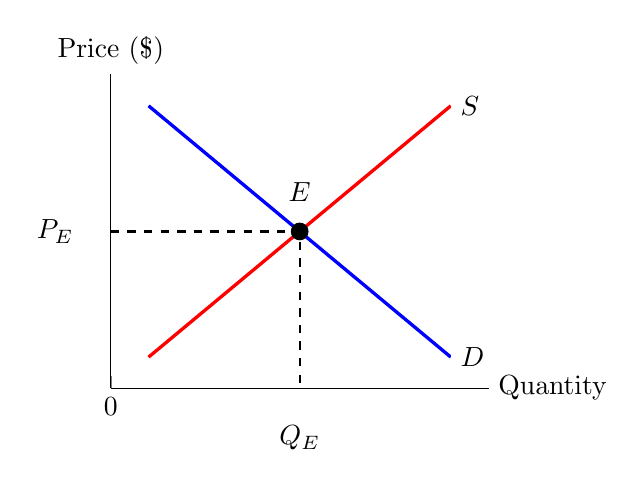
\begin{tikzpicture}
\begin{axis}[
scale = 0.7,
xmin = 0, xmax = 10,
ymin = 0.01, ymax = 10,
axis lines* = left,
xtick = {0}, ytick = \empty, 
clip = false,
]
% Supply and demand curves
\addplot[color = blue, very thick] coordinates {(1, 9) (9, 1)};
\addplot[color = red, very thick] coordinates {(1, 1) (9, 9)};

% Dashed lines
\addplot[color = black, dashed, thick] coordinates {(0, 5) (5, 5) (5, 0)};

% Coordinate points
\addplot[color = black, mark = *, only marks, mark size = 3pt] coordinates {(5, 5)};

% Labels
\node [right] at (current axis.right of origin) {Quantity};
\node [above] at (current axis.above origin) {Price (\$)};
\node [above = 5pt, fill = white] at (5, 5.2) {$E$};
\node [left = 10pt] at (0, 5) {$P_E$};
\node [below = 10pt] at (5, 0) {$Q_E$};
\node [right, fill = white] at (9, 1) {$D$};
\node [right, fill = white] at (9, 9) {$S$};
\end{axis}
\end{tikzpicture}
\caption{Simple Supply and Demand}
\label{fig:supdem}
\end{center}
\end{figure}

In ~\ref{fig:supdem}, point $E$ is the equilibrium point. It is as the point where the two lines intersect. Make sure to realize that these type of econ graphs often assume that the market is a perfectly competitive. Only in equilibriumis quantity supplied equal to quantity demanded. The market will come to rest at equilibrium unless there is a outside force. 

\begin{example}
    With equilibrium, there also exists disequlibrium, which is when the market is not at its stable state. It usually is either a surplus or a shortage, and can be resolved with changes. 
    \textbf{Surplus} is when demand shifts, and supply has not compensated yet. This leads to a surplus of goods, which is often solved by lowering the price. 
    \textbf{Shortage} is when supply shifts to the left, which is solved by raising the price. 
\end{example}

Another part of supply and demand graphs, is double shifts. Double shifts is when both supply and demand are shifted in directions, and cause the equilibrium point to be moved completely. Each teacher recommends doing this in different ways, but the best rule of thumb is to do the shifts in two different graphs, compare price and quantity and determine how it would move. You could get away with doing it all in one graph, but it depends on your teacher or if the collegeboard allows it. Two graphs is always a safe bet if you dont know which one to go with. 

Instead of doing a random example, lets model this with Toyota RAV4s. Toyota RAV4s are expected to rise 10\% after the new year. Create two different graphs, and analyze them to answer the questions:
\begin{itemize}
    \item What can you conclude about the current price of RAV4s?
    \item What can you conclude about the current quantity of RAV4s being bought and sold?
\end{itemize}

So lets reason this out: If the price is \textbf{expected} to go up after the new year, consumers will want to purchase now. Suppliers will attempt to store and wait for the new year to sell at a higher price. 

\begin{figure}[!h]
\begin{center}
\hspace*{-3cm}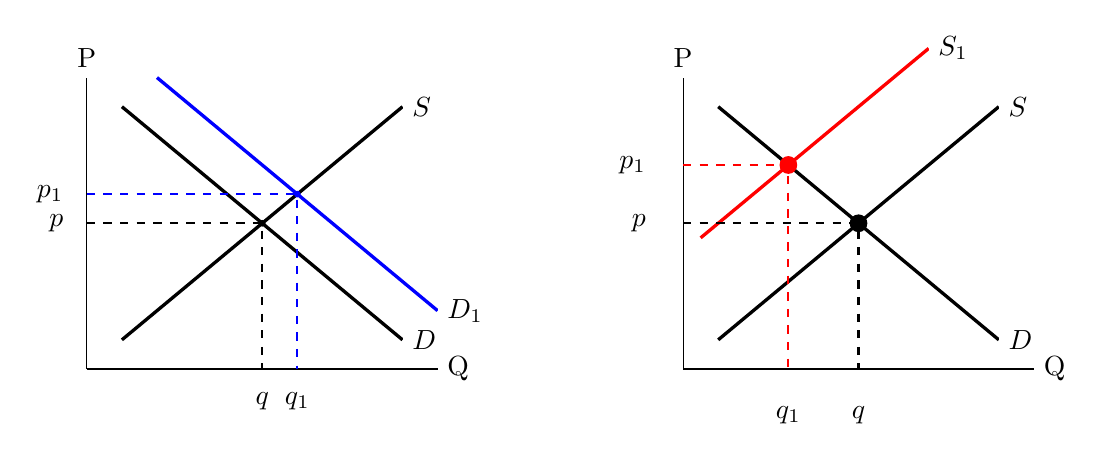
\begin{tikzpicture}
\begin{axis}[
scale = 0.65, 
xmin = 0, xmax = 10,
ymin = 0, ymax = 10,
axis lines* = left,
xtick = \empty, ytick = \empty,
clip = false,
]
\addplot[color = black, very thick] coordinates {(1,9) (9,1)};
\addplot[color = black, very thick] coordinates {(1,1) (9,9)};
\addplot[color = blue, very thick] coordinates {(2,10) (10,2)};
% Dashed Lines
\addplot[color = black, dashed, thick] coordinates {(0,5) (5,5) (5,0)};
\addplot[color = blue, dashed, thick] coordinates {(0,6) (6,6) (6,0)};
% Points
\addplot[color = black, mark = *, only marks, mark size = 1pt] coordinates {(5,5)};
\addplot[color = blue, mark = *, only marks, mark size = 1pt] coordinates {(6,6)};
% Labels
\node [right] at (current axis.right of origin) {Q};
\node [above] at (current axis.above origin) {P};
\node [left = 5pt] at (0,5) {$p$};
\node [below = 5pt] at (5,0) {$q$};
\node [left = 5pt] at (0,6) {$p_1$};
\node [below = 5pt] at (6,0) {$q_1$};
\node [right, fill = white] at (9,1) {$D$};
\node [right, fill = white] at (9,9) {$S$};
\node [right, fill = white] at (10,2) {$D_1$};
\end{axis}
\begin{axis}[
scale = 0.65, 
xmin = 0, xmax = 10,
ymin = 0, ymax = 10,
axis lines* = left,
xtick = \empty, ytick = \empty,
clip = false,
shift = {(axis cs: 17, 0)},
]
\addplot[color = black, very thick] coordinates {(1,9) (9,1)};
\addplot[color = black, very thick] coordinates {(1,1) (9,9)};
\addplot[color = red, very thick] coordinates {(0.5,4.5) (7,11)};
%\addplot[color = blue, very thick] coordinates {(2,10) (10,2)};
% Dashed Lines
\addplot[color = black, dashed, thick] coordinates {(0,5) (5,5) (5,0)};
\addplot[color = red, dashed, thick] coordinates {(0,7) (3,7) (3,0)};
% Points
\addplot[color = black, mark = *, only marks, mark size = 3pt] coordinates {(5,5)};
\addplot[color = red, mark = *, only marks, mark size = 3pt] coordinates {(3,7)};
% Labels
\node [right] at (current axis.right of origin) {Q};
\node [above] at (current axis.above origin) {P};
\node [left = 10pt] at (0,5) {$p$};
\node [below = 10pt] at (5,0) {$q$};
\node [left = 10pt] at (0,7) {$p_1$};
\node [below = 10pt] at (3,0) {$q_1$};
\node [right, fill = white] at (9,1) {$D$};
\node [right, fill = white] at (9,9) {$S$};
\node [right, fill = white] at (7,11) {$S_1$};
\end{axis}
\end{tikzpicture}\hspace*{-3cm}
\caption{Market for RAV4}
\label{fig:rav4}
\end{center}
\end{figure}

Now we can analyze the graphs, and focus on them one at a time. With the increase in demand, price went up and quantity went up. With decrease in supply, price went up and quantity went down. 
\begin{itemize}
    \item Since price increases in both graphs, it is certain that \textbf{price will increase}
    \item Since quantity went up in one graph, and down in another, that means \textbf{quantity is indeterminate}
\end{itemize}

